\documentclass{article}
\usepackage{amsmath,amssymb,amsthm,latexsym,paralist}
\usepackage{tikz, algorithm, algpseudocode}

\theoremstyle{definition}
\newtheorem{problem}{Problem}
\newtheorem*{solution}{Solution}
\newtheorem*{resources}{Resources}

\newcommand{\name}[1]{\noindent\textbf{Name: {#1}}}
\newcommand{\honor}{\noindent On my honor, as an Aggie, I have neither
  given nor received any unauthorized aid on any portion of the
  academic work included in this assignment. Furthermore, I have
  disclosed all resources (people, books, web sites, etc.) that have
  been used to prepare this homework. \\[1ex]
 \textbf{Signature:} \underline{\hspace*{5cm}} }

\newcommand{\checklist}{\noindent\textbf{Checklist:}
\begin{compactitem}[$\Box$] 
\item Did you add your name? 
\item Did you disclose all resources that you have used? \\
(This includes all people, books, websites, etc. that you have consulted)
\item Did you sign that you followed the Aggie honor code? 
\item Did you solve all problems? 
\item Did you write the solution in your own words? 
\item Did you submit the pdf file of your homework?
\end{compactitem}
}

\newcommand{\problemset}[1]{\begin{center}\textbf{Problem Set #1}\end{center}}
\newcommand{\duedate}[1]{\begin{quote}\textbf{Due dates:} Typeset your
    solution in \LaTeX{}. Electronic
    submission of the resulting .pdf file of this homework is due on
    \textbf{#1} on canvas. If your submission cannot be checked by
    turnitin, then it will not be graded.\end{quote} }

\newcommand{\N}{\mathbf{N}}
\newcommand{\R}{\mathbf{R}}
\newcommand{\Z}{\mathbf{Z}}

\usepackage{tikz}
\usetikzlibrary{positioning}
\tikzset{face/.style={scale=0.5,shape=circle,minimum size=4ex,shading=radial,outer sep=0pt,
        inner color=white!50!yellow,outer color= yellow!70!orange}}

\newcommand{\aha}{%

\begin{tikzpicture}[scale=0.5]
     \node[face] {}; 
     \draw[fill=white] (-1ex,0ex) ..controls (-0.5ex,0.2ex)and(0.5ex,0.2ex)..
        (1ex,0.0ex) ..controls ( 1.5ex,1.5ex)and( 0.2ex,1.7ex)..
        (0ex,0.4ex) ..controls (-0.2ex,1.7ex)and(-1.5ex,1.5ex)..
        (-1ex,0ex)--cycle;
    \fill[shift={(0.5ex,0.5ex)},rotate=80] 
       (0,0) ellipse (0.3ex and 0.15ex);
  \fill[shift={(-0.5ex,0.5ex)},rotate=100] 
       (0,0) ellipse (0.3ex and 0.15ex);
  \draw[] (-1.5ex,-0.5ex)
               ..controls (-0.7ex,-1.7ex)and(0.7ex,-1.7ex)..(1.5ex,-0.5ex);
\end{tikzpicture}
}

\newcommand{\confused}{%     

\begin{tikzpicture}[scale=0.5]
  \node[face] {}; 
\draw[fill=white] (-1ex,0ex) ..controls (-0.5ex,0.2ex)and(0.5ex,0.2ex)..
        (1ex,0.0ex) ..controls ( 1.5ex,1.5ex)and( 0.2ex,1.7ex)..
        (0ex,0.4ex) ..controls (-0.2ex,1.7ex)and(-1.5ex,1.5ex)..
        (-1ex,0ex)--cycle;
    \fill[shift={(0.5ex,0.5ex)},rotate=80] 
       (0,0) ellipse (0.3ex and 0.15ex);
  \fill[shift={(-0.5ex,0.5ex)},rotate=100] 
       (0,0) ellipse (0.3ex and 0.15ex);
  \draw[] (-1ex,-0.75ex)--(1ex,-1.25ex);
\end{tikzpicture}
}


\begin{document}
\problemset{2}
\duedate{Friday, Feb 3, before 11:59pm}
\name{(put your name here)}
\begin{resources} (All people, books, articles, web pages, etc. that
  have been consulted when producing your answers to this homework)
\end{resources}
\honor

\newpage

\noindent\textbf{Problem A.} Solve the following five subproblems. 

\begin{problem}[20 points] 
Give a self-contained proof of the fact that 
$$\log_2(n!)\in \Theta(n\log n).$$
[For part of your argument, you can use results that were given in the
lecture, but you should write up the proof in your own words. Make
sure that you write it in complete sentences, even when the sentence
contains formulas. A good check is to read out the entire solution
aloud. It should read smoothly.] 
\end{problem}
\begin{solution}
\end{solution}  

\newpage
\begin{problem}[20 points] 
  Amelia attempted to solve $n$ algorithmic problems. She wrote down
  one problem per page in her journal and marked the page with
  \confused when she was unable to solve the problem and with \aha
  when she was able to solve it. So the pages of her journal look like
  this: 
$$ 
\begin{array}{|c|c|c|c|c|c|c|c|}
\hline
\vphantom{\Big|}\confused&\confused&\confused&\aha&\confused&\aha&\confused&\aha\\
\hline
\end{array}
$$
Use the decision tree method to show that any algorithm to find a page with an
\aha smiley on has to look at all $n$ pages in the worst case. 
\end{problem}
\begin{solution}
Amelia's journal pages can be searched through the use of a binary search tree. Each 'level' of the tree 
would correspond to an individual page, so the height of the tree $h$ is equivalent to the $n$ number of 
pages. Each node but the last should have one child node for \aha if the problem was solved and the 
other for \confused if she was unable to solve it. The \aha nodes are leaf nodes, since the search may 
conclude once a solved page is found. \confused nodes would continue the binary tree for as many levels
as there are pages used. Consider the example provided, where Amelia has 8 pages she wishes to search
through. The resulting decision tree would appear as follows: \\
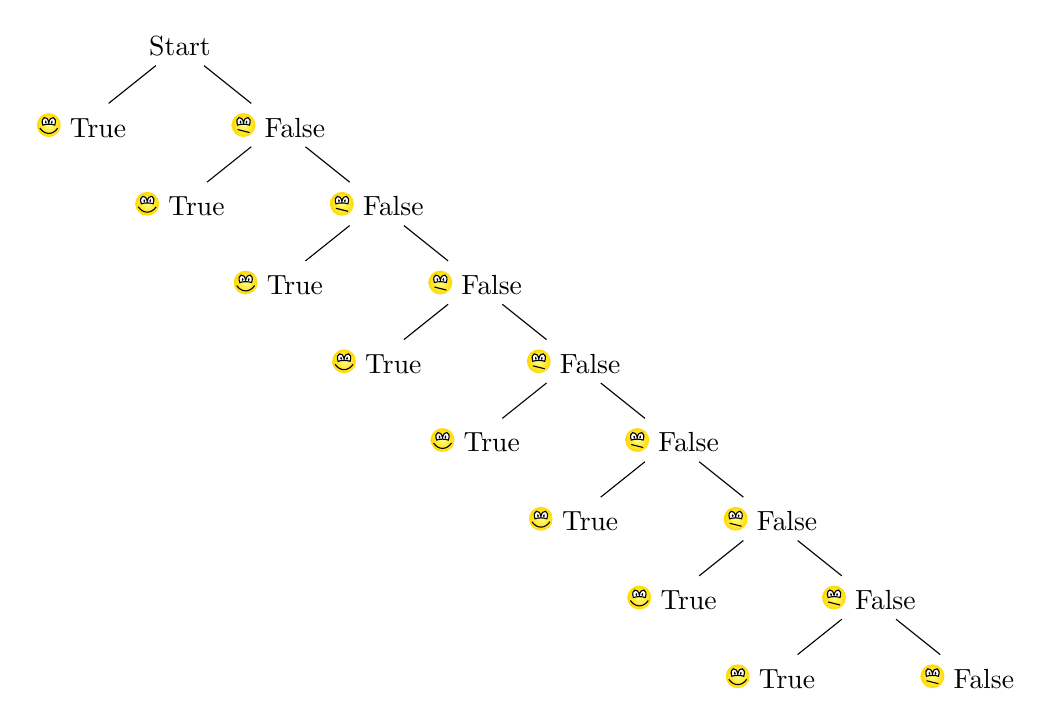
\begin{tikzpicture}[shift={(-5,0)}]
\node{Start}
[sibling distance=2.5cm,
level distance=1cm]
child{node{\aha True}}
child{node{\confused False}
 child{node{\aha True}}
 child{node{\confused False}
  child{node{\aha True}}
  child{node{\confused False}
   child{node{\aha True}}
   child{node{\confused False}
    child{node{\aha True}}
    child{node{\confused False}
     child{node{\aha True}}
     child{node{\confused False}
      child{node{\aha True}}
      child{node{\confused False}
       child{node{\aha True}}
       child{node{\confused False}
       }
      }
     }
    }
   }
  }
 }
};
\end{tikzpicture}
In the worst case, one of two situations are possible; Amelia was only able to solve the $nth$ problem, or none
at all. The decision tree must then visit each of the $n$ nodes down the tree until it reaches the $nth$ node (page). 
The status \mbox{$(\aha/\confused)$} of this last page is inconsequential for this question, as we have already had to look
at each of the $n$ nodes anyway.
\end{solution}  

\newpage
\begin{problem}[20 points] 
  Amelia attempted to solve $n$ algorithmic problems. She wrote down
  one problem per page in her journal and marked the page with
  \confused when she was unable to solve the problem and with \aha
  when she was able to solve it. So the pages of her journal look like
  this: 
$$ 
\begin{array}{|c|c|c|c|c|c|c|c|}
\hline
\vphantom{\Big|}\confused&\confused&\confused&\aha&\confused&\aha&\confused&\aha\\
\hline
\end{array}
$$
Use an adversary method to show that any method to find a page with a
\aha smiley on it might have to look at all $n$ pages. 
\end{problem}
\begin{solution}
Under an adversarial method, our adversary is able to control the observation (input) that the algorithm sees and
bases its actions on. The adversary is looking to slow the algorithm down as much as possible, and the algorithm
cannot see what is actually written on the page(s). It must, unfortunately, rely only on what the adversary says is
on the page. There is also nothing stopping the adversary from reordering the pages so that all of the \confused unsolved
pages are at the front, while all of the \aha solved pages are pushed to the back. The absolute worst case for the 
algorithm is, as previously described, when all but the last problem are \confused unsolved. Thus, as the algorithm 
asks the adversary if a page is solved, the adversary will naturally reply with a 'no'. Upon reaching the $nth$ page,
the adversary can answer either way as it has already succeeded in its goal of generating a worst case. The 
algorithm has had to observe each of the $n$ pages.
\end{solution}  

\newpage
\begin{problem}[20 points] 
  Amelia attempted to solve $n$ algorithmic problems, where $n$ is an
  odd number. She wrote down one problem per page in her journal and
  marked the page with \confused when she was unable to solve the
  problem and with \aha when she was able to solve it. Suppose that we
  want to find the pattern $\confused\aha$, where she was unable to
  solve a problem, but was able to solve the subsequent problem. 

  Find an algorithm that always looks at fewer than $n$ pages but is
  able to correctly find the pattern when it exists. [Hint: First look
  at all even pages.] 
\end{problem}
\begin{solution}
\begin{algorithm}
\caption{Pattern Search}
\begin{algorithmic} \\
\For{$i \leftarrow 2$ to $n$ number of pages, $step = 2$}
\If{page[i] contains TRUE}
\If{page[i-1] contains FALSE}
\Return ``pattern found at $(i-1)$''
\EndIf
\ElsIf{page[i] contains FALSE}
\If{page[i+1] contains TRUE}
\Return ``pattern found at $i$''
\EndIf
\EndIf
\EndFor
\If{pattern not found}
\Return ``pattern doesn't exist''
\EndIf
\end{algorithmic}
\end{algorithm}
\end{solution}  

\newpage
\begin{problem}[20 points]
Suppose that we are given a sorted array $A[1..n]$ of $n$ numbers. Our
goal is to determine whether or not the array $A$ contains
duplicate elements. We will limit ourselves to algorithms that use only the spaceship
operator \verb|<=>| for comparisons, where 
\begin{verbatim}
a <=> b :=
  if a < b then return -1
  if a = b then return  0
  if a > b then return  1
  if a and b are not comparable then return nil
\end{verbatim}
No other methods will be used to compare or inspect elements of the
array. 
\begin{enumerate}[(a)]
\item Give an efficient (optimal) comparison-based algorithm that decides
  whether $A[1..n]$ contains duplicates using the spaceship operator
  for comparisons. 
\item Use an adversarial argument to show that no algorithm can solve
  the problem with fewer calls to the comparison operator \verb|<=>|
  than the algorithm that you gave in (a). 
\end{enumerate}
\end{problem}
\begin{solution} :
\begin{algorithm}
\caption{Finding duplicates in an array}
\begin{algorithmic} \\
\For{$i \leftarrow 0$ to $n-1$}
    \If{$A[i] \leftrightarrow A[i + 1] == 0$}
        \Return ``duplicate elements found at $i$ and $i+1$''
        \State \textbf{end}
    \EndIf
\EndFor
\State \textbf{else} Output ``duplicate elements do not exist''
\end{algorithmic}
\end{algorithm} \\
(a)\newline
In Problem 4, the binary format of the pages (\aha or \confused) allowed for a very efficient search that did not have to
look at all $n$ pages. The value of a page meant the algorithm only had to look to one direction from the current page for
its operation. This problem is not as friendly, as equality could come from either side of a given point in the array. Since the
array is already sorted, we know that any equal elements will be next to each other. Using only the spaceship operator, it
would therefore seem that the most optimal solution is to iterate once through the first $n-1$ elements and compare to the
next element. \\
(b) \\
Before, the worst case of the journal page search arose when all of Amelia's pages were \confused unsolved or only the last
page was \aha solved. Similarly, the worst case here occurs when either none of the elements are equal or only the last two are.
Say our adversary creates the following array for the algorithm: 
$$
\begin{array}{|c|c|c|c|c|}
\hline
\vphantom{\Big|}2&4&6&8&8\\
\hline
\end{array}
$$
The only equal values occur in A[4] and A[5], the final two indexes in the array. This means that the algorithm will have to make
all $n-1=4$ comparisons available to find any equality, a worst case for this algorithm. 
\end{solution}

\medskip
\goodbreak
\checklist
\end{document}
